\documentclass[border=2mm]{standalone}
\usepackage[svgnames]{xcolor}
\usepackage{tikz}
\usetikzlibrary{calc,arrows.meta}

\tikzset{
	doohicky/.pic = {
		\fill[color=Aqua,rounded corners] (-15pt,-11pt) rectangle (15pt,-1pt);
		\fill[color=yellow] (-10pt,-6pt) circle[radius=4pt]
					    (0pt,-6pt) circle[radius=4pt]
					    (10pt,-6pt) circle[radius=4pt];
	}
}

\begin{document}
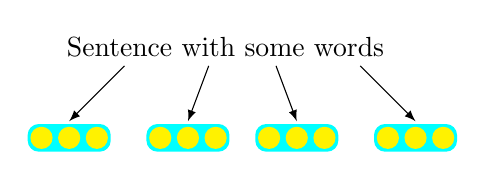
\begin{tikzpicture}
	\node (A) {Sentence with some words};
	\draw[-latex] ($(A.south west)!.2!(A.south east)$) -- ++(-20pt,-20pt) pic{doohicky};
	\draw[-latex] ($(A.south west)!.45!(A.south east)$) -- ++(-7.5pt,-20pt) pic{doohicky};
	\draw[-latex] ($(A.south west)!.65!(A.south east)$) -- ++(7.5pt,-20pt) pic{doohicky};
	\draw[-latex] ($(A.south west)!.9!(A.south east)$) -- ++(20pt,-20pt) pic{doohicky};
\end{tikzpicture}
\end{document}